% !TEX program = xelatex
% CH304 化工熱力學 期末報告：企業顧問報告——非理想混合系統之相平衡與能量分析（Ethanol/Water）
% 結構依課程規定 Part I--V；正文 6--10 頁（不含附錄）。所有數字由 calc/make_numbers.py 產生於 numbers.tex。
\documentclass[UTF8,a4paper,11pt,fontset=none,zihao=-4]{ctexart}

% ------------------------------------------------------------------ fonts
\usepackage{amsmath,amssymb}
\usepackage{unicode-math}
\setmainfont{Latin Modern Roman}
\setsansfont{Latin Modern Sans}
\setmonofont{Latin Modern Mono}
\setmathfont{Latin Modern Math}
\setCJKmainfont{Noto Serif CJK TC}[BoldFont={Noto Serif CJK TC Black},ItalicFont={AR PL KaitiM Big5}]
\setCJKsansfont{Noto Sans CJK TC}[BoldFont={Noto Sans CJK TC Bold}]
\setCJKmonofont{Noto Sans CJK TC}

% ------------------------------------------------------------------ layout
\usepackage[top=2.2cm,bottom=2.2cm,left=2.3cm,right=2.3cm,headheight=14pt]{geometry}
\linespread{1.16}
\usepackage{xcolor}
\definecolor{accent}{HTML}{1B4F8A}
\definecolor{warn}{HTML}{B91C1C}
\definecolor{soft}{HTML}{F3F6FA}
\usepackage{graphicx,booktabs,multirow,makecell,array,threeparttable,tabularx}
\usepackage{float}
\usepackage[labelfont=bf,font=small,labelsep=quad,skip=4pt]{caption}
\usepackage{siunitx}
\sisetup{group-separator={,},group-minimum-digits=4,detect-all}
\usepackage{enumitem}
\setlist{itemsep=1pt,topsep=3pt,parsep=0pt,leftmargin=2em}
\usepackage{multicol}
\usepackage{tikz}
\usetikzlibrary{arrows.meta,positioning,calc}
\usepackage[most]{tcolorbox}
\usepackage{fancyhdr}
\usepackage{titletoc}
\usepackage{url}
\usepackage[hidelinks,bookmarksnumbered]{hyperref}
\usepackage[nameinlink]{cleveref}
\crefname{figure}{圖}{圖}\Crefname{figure}{圖}{圖}
\crefname{table}{表}{表}\Crefname{table}{表}{表}
\crefname{equation}{式}{式}\Crefname{equation}{式}{式}
\creflabelformat{equation}{(#2#1#3)}
\newcommand{\crefpairconjunction}{、}\newcommand{\crefmiddleconjunction}{、}
\newcommand{\creflastconjunction}{、}\newcommand{\crefrangeconjunction}{--}
\setlength{\emergencystretch}{3em}
\setlength{\textfloatsep}{8pt plus 2pt minus 2pt}
\setlength{\floatsep}{8pt plus 2pt minus 2pt}
\setlength{\intextsep}{8pt plus 2pt minus 2pt}

% Part I--V headings; figures/tables/equations numbered by part in Arabic (圖 3.1 = Part III 第 1 張)
\ctexset{
  section={format=\Large\sffamily\bfseries\color{accent}\raggedright, name={Part~,\,｜}, number=\Roman{section},
           beforeskip=1.4ex plus .3ex, afterskip=0.8ex},
  subsection={format=\large\sffamily\bfseries\raggedright, beforeskip=1.0ex, afterskip=.5ex},
  subsubsection={format=\normalsize\sffamily\bfseries\raggedright, beforeskip=.8ex, afterskip=.3ex},
  paragraph={format=\normalsize\sffamily\bfseries, afterskip=.6em},
  appendix={name={附錄\,},number=\Alph{section}},
  contentsname={目\quad 錄},
  figurename={圖},tablename={表},
}
\renewcommand{\thesubsection}{\arabic{section}.\arabic{subsection}}
\numberwithin{equation}{section}\renewcommand{\theequation}{\arabic{section}.\arabic{equation}}
\numberwithin{figure}{section}\renewcommand{\thefigure}{\arabic{section}.\arabic{figure}}
\numberwithin{table}{section}\renewcommand{\thetable}{\arabic{section}.\arabic{table}}

\pagestyle{fancy}
\fancyhf{}
\fancyhead[L]{\small\sffamily\color{gray}企業顧問報告：乙醇--水系統之相平衡與能量分析}
\fancyhead[R]{\small\sffamily\color{gray}CH304 化工熱力學}
\fancyfoot[C]{\small\thepage}
\renewcommand{\headrulewidth}{0.4pt}

\newtcolorbox{keybox}[1][]{enhanced,colback=soft,colframe=accent,boxrule=0.6pt,arc=2pt,
  left=6pt,right=6pt,top=3pt,bottom=3pt,fonttitle=\sffamily\bfseries,title={#1}}
\newtcolorbox{notebox}[1][]{enhanced,colback=white,colframe=gray!60,boxrule=0.4pt,arc=2pt,
  left=6pt,right=6pt,top=2pt,bottom=2pt,fonttitle=\sffamily\bfseries\small,coltitle=black,colbacktitle=gray!12,title={#1}}
\newtcolorbox{answerbox}{enhanced,colback=white,colframe=accent!60,boxrule=0.5pt,arc=2pt,left=6pt,right=6pt,top=2pt,bottom=2pt,
  borderline west={2.5pt}{0pt}{accent}}

\makeatletter
\newcommand{\inputtab}[1]{\@@input #1 }
\makeatother
\newcommand{\dd}{\mathrm{d}}
\newcommand{\sat}{\mathrm{sat}}

% ------------------------------------------------------------------ editable front matter
\newcommand{\GroupName}{第二組}
% 組員（5--6 人）：請直接改下列六行；不足六人時刪除多餘行
\newcommand{\MemberList}{%
（姓名）\quad（學號）\\
（姓名）\quad（學號）\\
（姓名）\quad（學號）\\
（姓名）\quad（學號）\\
（姓名）\quad（學號）\\
（姓名）\quad（學號）}
\newcommand{\Instructor}{Prof.\ Chi-Wei Lan}
\newcommand{\ReportDate}{\today}

% Auto-generated by calc/make_numbers.py from results/results.json -- do not edit by hand
\newcommand{\nTbEtOH}{78.30}
\newcommand{\nTbWater}{99.97}
\newcommand{\ndTmax}{11.1}
\newcommand{\ndTmaxX}{0.16}
\newcommand{\ndTmid}{7.1}
\newcommand{\nxAz}{0.8947}
\newcommand{\nTAz}{78.14}
\newcommand{\nwAz}{95.6}
\newcommand{\nxAzVir}{0.8863}
\newcommand{\nxAzFit}{0.8915}
\newcommand{\nxAzVL}{0.8921}
\newcommand{\nxAzExp}{0.895}
\newcommand{\nTAzExp}{78.11}
\newcommand{\ngOneInf}{5.70}
\newcommand{\ngTwoInf}{2.58}
\newcommand{\nalphaMax}{12.6}
\newcommand{\nalphaIdLo}{2.23}
\newcommand{\nalphaIdHi}{2.29}
\newcommand{\nvlA}{1.700}
\newcommand{\nvlAse}{0.013}
\newcommand{\nvlB}{0.953}
\newcommand{\nvlBse}{0.002}
\newcommand{\nvlChi}{0.22}
\newcommand{\nvlCorr}{\ensuremath{-}0.73}
\newcommand{\nnrA}{\ensuremath{-}37.5}
\newcommand{\nnrAse}{2.9}
\newcommand{\nnrB}{640.6}
\newcommand{\nnrBse}{7.6}
\newcommand{\nnrChi}{0.33}
\newcommand{\nnrCorr}{\ensuremath{-}0.978}
\newcommand{\nnPts}{21}
\newcommand{\nherD}{3.7}
\newcommand{\nherJ}{9.3}
\newcommand{\nBee}{\ensuremath{-}789}
\newcommand{\nBww}{\ensuremath{-}581}
\newcommand{\nBew}{\ensuremath{-}658}
\newcommand{\nvirdT}{0.06}
\newcommand{\nvirdy}{0.0043}
\newcommand{\ngEmax}{908}
\newcommand{\ngEmaxX}{0.43}
\newcommand{\nhEmin}{\ensuremath{-}230}
\newcommand{\nhEminX}{0.21}
\newcommand{\nhEmax}{67}
\newcommand{\nhEmaxX}{0.81}
\newcommand{\nhEzero}{0.60}
\newcommand{\nTsEmin}{\ensuremath{-}1060}
\newcommand{\nTsEminX}{0.35}
\newcommand{\ncpEmax}{1.8}
\newcommand{\nhEfitMax}{639}
\newcommand{\nhEfitMaxTwoNineEight}{556}
\newcommand{\nhEtwoNineEightMin}{\ensuremath{-}298}
\newcommand{\nhEtwoNineEightMinX}{0.25}
\newcommand{\nhEtwoNineEightAtExp}{\ensuremath{-}274}
\newcommand{\nhEratio}{0.56}
\newcommand{\ndHratio}{0.949}
\newcommand{\nhEzeroTwoNineEight}{0.81}
\newcommand{\nhEzeroThreeSevenThree}{0.54}
\newcommand{\ndTadExp}{9.5}
\newcommand{\ndTadNRTL}{3.4}
\newcommand{\ncpMix}{81.6}
\newcommand{\nTrefC}{78.14}
\newcommand{\naadTAAD}{5.49}
\newcommand{\nmaxTAAD}{11.23}
\newcommand{\naadyAAD}{0.0924}
\newcommand{\nmaxyAAD}{0.260}
\newcommand{\nbiasTAAD}{5.49}
\newcommand{\naadTVL}{0.080}
\newcommand{\nmaxTVL}{0.35}
\newcommand{\naadyVL}{0.0031}
\newcommand{\nmaxyVL}{0.013}
\newcommand{\nbiasTVL}{0.047}
\newcommand{\naadTNL}{0.072}
\newcommand{\nmaxTNL}{0.28}
\newcommand{\naadyNL}{0.0027}
\newcommand{\nmaxyNL}{0.012}
\newcommand{\nbiasTNL}{0.044}
\newcommand{\naadTNF}{0.116}
\newcommand{\nmaxTNF}{0.61}
\newcommand{\naadyNF}{0.0039}
\newcommand{\nmaxyNF}{0.020}
\newcommand{\nbiasTNF}{0.080}
\newcommand{\naadTNV}{0.078}
\newcommand{\nmaxTNV}{0.30}
\newcommand{\naadyNV}{0.0042}
\newcommand{\nmaxyNV}{0.016}
\newcommand{\nbiasTNV}{0.013}
\newcommand{\nxF}{0.10}
\newcommand{\nxD}{0.85}
\newcommand{\nxB}{0.002}
\newcommand{\nFflow}{100}
\newcommand{\nRR}{1.3}
\newcommand{\nRminId}{6.58}
\newcommand{\nRId}{8.55}
\newcommand{\nNminId}{10}
\newcommand{\nNId}{24}
\newcommand{\nNFId}{7}
\newcommand{\nVId}{110.4}
\newcommand{\nQBId}{1246}
\newcommand{\nQCId}{1192}
\newcommand{\nEspId}{9.92}
\newcommand{\npinchId}{0.100}
\newcommand{\nTtopId}{82.8}
\newcommand{\nTbotId}{99.9}
\newcommand{\nRminNl}{1.89}
\newcommand{\nRNl}{2.46}
\newcommand{\nNminNl}{11}
\newcommand{\nNNl}{30}
\newcommand{\nNFNl}{27}
\newcommand{\nVNl}{39.9}
\newcommand{\nQBNl}{451}
\newcommand{\nQCNl}{431}
\newcommand{\nEspNl}{3.59}
\newcommand{\npinchNl}{0.754}
\newcommand{\nTtopNl}{78.2}
\newcommand{\nTbotNl}{99.8}
\newcommand{\nRminNf}{1.96}
\newcommand{\nRNf}{2.55}
\newcommand{\nNminNf}{12}
\newcommand{\nNNf}{31}
\newcommand{\nNFNf}{27}
\newcommand{\nVNf}{41.1}
\newcommand{\nQBNf}{464}
\newcommand{\nQCNf}{443}
\newcommand{\nEspNf}{3.69}
\newcommand{\npinchNf}{0.758}
\newcommand{\nTtopNf}{78.2}
\newcommand{\nTbotNf}{99.8}
\newcommand{\nDflow}{11.56}
\newcommand{\nQBratio}{2.76}
\newcommand{\nxDach}{0.826}
\newcommand{\nxBach}{0.0051}
\newcommand{\nlossRatio}{2.6}
\newcommand{\nRneed}{68}
\newcommand{\nQBneed}{8948}
\newcommand{\nTshiftMax}{18.5}
\newcommand{\nRminIdNinetyNine}{8.04}
\newcommand{\nsensRa}{2.08}
\newcommand{\nsensNa}{50}
\newcommand{\nsensNFa}{47}
\newcommand{\nsensQa}{402}
\newcommand{\nsensRb}{2.27}
\newcommand{\nsensNb}{36}
\newcommand{\nsensNFb}{33}
\newcommand{\nsensQb}{426}
\newcommand{\nsensRc}{2.46}
\newcommand{\nsensNc}{30}
\newcommand{\nsensNFc}{27}
\newcommand{\nsensQc}{451}
\newcommand{\nsensRd}{2.83}
\newcommand{\nsensNd}{24}
\newcommand{\nsensNFd}{21}
\newcommand{\nsensQd}{500}
\newcommand{\nsensRe}{3.78}
\newcommand{\nsensNe}{19}
\newcommand{\nsensNFe}{16}
\newcommand{\nsensQe}{624}
\newcommand{\nxAzPTen}{0.943}
\newcommand{\nTAzPTen}{29.2}
\newcommand{\nxAzPTwenty}{0.930}
\newcommand{\nTAzPTwenty}{42.1}
\newcommand{\nxAzPFifty}{0.910}
\newcommand{\nTAzPFifty}{61.3}
\newcommand{\nxAzPAtm}{0.895}
\newcommand{\nTAzPAtm}{78.1}
\newcommand{\nxAzPThreeHundred}{0.870}
\newcommand{\nTAzPThreeHundred}{108.2}
\newcommand{\nxAzPFive}{0.954}
\newcommand{\nTAzPFive}{17.4}
\newcommand{\npsdDxa}{0.035}
\newcommand{\npsdReca}{2.0}
\newcommand{\npsdDxb}{0.048}
\newcommand{\npsdRecb}{1.2}
\newcommand{\npsdDxc}{0.025}
\newcommand{\npsdRecc}{4.3}
\newcommand{\npsdDxd}{0.059}
\newcommand{\npsdRecd}{1.2}
\newcommand{\npsatDevMax}{0.7}
\newcommand{\npsatDevHi}{1.2}
\newcommand{\nTbEtOHeos}{78.42}
\newcommand{\nsTtopSeventy}{78.59}
\newcommand{\nsTtopEightyFive}{78.17}
\newcommand{\nsdTtop}{0.44}
\newcommand{\nsdTdxDil}{107}
\newcommand{\nsdTdxTop}{2.8}
\newcommand{\nsdTdP}{0.25}
\newcommand{\nsdxEquiv}{0.09}
\newcommand{\nsdxazdlnP}{0.022}
\newcommand{\nsTdilTwo}{94.8}
\newcommand{\nsTdilTen}{86.2}
\newcommand{\negN}{33}
\newcommand{\negNrel}{32}
\newcommand{\negNhi}{5}
\newcommand{\negXpLo}{0.89}
\newcommand{\negXpHi}{0.96}
\newcommand{\negXegLo}{0.28}
\newcommand{\negXegHi}{0.56}
\newcommand{\negAlphaLo}{1.51}
\newcommand{\negAlphaHi}{2.24}
\newcommand{\negAlphaBinLo}{0.93}
\newcommand{\negAlphaBinHi}{1.01}
\newcommand{\negEnhLo}{0.86}
\newcommand{\negEnhHi}{0.94}


\begin{document}

% ================================================================== cover
\begin{titlepage}
\thispagestyle{empty}
\setlength{\parindent}{0pt}
\begin{tikzpicture}[remember picture,overlay]
  \fill[accent] (current page.north west) rectangle ([yshift=-0.9cm]current page.north east);
  \fill[accent!15] ([yshift=-0.9cm]current page.north west) rectangle ([yshift=-1.05cm]current page.north east);
\end{tikzpicture}
\vspace*{1.8cm}
{\sffamily\color{accent}\large Chemical Engineering Thermodynamics\quad 化工熱力學 期末報告}\par
\vspace{0.7cm}
{\sffamily\bfseries\fontsize{23}{31}\selectfont 企業顧問報告：\\[2pt]非理想混合系統之相平衡與能量分析}\par
\vspace{0.35cm}
{\sffamily\Large 指定系統：Ethanol (1) / Water (2)，101.325\,kPa}\par
\vspace{0.4cm}
{\large Consulting Report: Phase Equilibrium and Energy Analysis of a Non-ideal Mixture}\par
\vspace{1.1cm}
\begin{tcolorbox}[enhanced,colback=soft,colframe=soft,arc=2pt,left=10pt,right=10pt,top=6pt,bottom=6pt]
\small
\begin{tabular}{@{}p{2.6cm}>{\raggedright\arraybackslash}p{11.2cm}@{}}
委託單位 & 精細化學品與生技材料公司（溶劑回收蒸餾單元）\\
指定理論基礎 & S.\,I.\ Sandler, \textit{Chemical, Biochemical, and Engineering Thermodynamics}, 5th ed., Ch.\,6--10\\
熱力學模型 & Raoult 定律（理想）與 NRTL（非理想）；$\gamma$--$\phi$ 相平衡\\
參數來源 & NRTL：Aspen Plus/DDB 資料庫（Beneke 等 2013）；蒸氣壓：NIST、IAPWS-95\\
驗證數據 & Kamihama 等（2012）等壓 VLE；Larkin（1975）、Ott 等（1986）量熱數據\\
計算工具 & Python（NumPy／SciPy／Matplotlib），程式與數據見附錄 G
\end{tabular}
\end{tcolorbox}
\vfill
\begin{tabular}{@{}l l@{}}
\sffamily 組別 & \GroupName \\[3pt]
\sffamily 組員 & \begin{tabular}[t]{@{}l@{}}\MemberList\end{tabular} \\[3pt]
\sffamily 授課教師 & \Instructor \\[2pt]
\sffamily 日期 & \ReportDate
\end{tabular}
\end{titlepage}

% ================================================================== TOC
\pagenumbering{roman}
\begingroup
\titlecontents{section}[0em]{\addvspace{3pt}\bfseries}{\thecontentslabel\quad}{}{\hfill\contentspage}
\titlecontents{subsection}[3.2em]{}{\contentslabel{2.2em}}{}{\titlerule*[0.6pc]{.}\contentspage}
\small
\tableofcontents
\endgroup
\vspace{1.2em}
\begin{notebox}[報告結構與評分項目對照]
\small
\begin{tabularx}{\linewidth}{@{}lX@{}}
Part I（10\%） & 執行摘要：核心問題、理想溶液為何失效、改用 NRTL 後的設計改變、最重要的一項建議 \\
Part II（20\%） & 單元操作角色、涉及的相（VLE）、為何需要 fugacity／activity coefficient、相平衡條件 \\
Part III（30\%） & (A) NRTL 假設、$\tau_{ij}$ 與 $\alpha_{ij}$ 的物理意義、為何適用；(B) Raoult vs NRTL 的 $T$--$x$--$y$ 計算、比較圖、偏差最大區域與工程誤判 \\
Part IV（25\%） & NRTL 計算 $G^{E}$ 與 $\Delta H_{\mathrm{mix}}$、作圖、吸熱／放熱、對混合槽／溫控與塔能耗的影響 \\
Part V（15\%） & 製程合理性、最敏感的操作變數（$T$、$P$、組成）、改變操作條件／改用溶劑／分段操作的建議與熱力學理由 \\
附錄 A--G & 數據與方法細節、驗證統計、汽相修正、推導、塔設計細節、壓力效應、程式（不計入正文頁數）
\end{tabularx}
\end{notebox}
\clearpage
\pagenumbering{arabic}

% ================================================================== Part I
\section{執行摘要（Executive Summary）}\label{sec:exec}

\paragraph{委託背景與核心問題。}貴公司以常壓連續蒸餾塔從發酵／萃取上游的稀乙醇水溶液回收乙醇，並在進塔前以混合槽調配進料。原設計以\textbf{理想溶液（Raoult 定律）}計算相平衡，現場出現三個症狀：能耗預估嚴重偏差、操作溫度不穩、預期的分離沒有發生。本報告的結論是：三個症狀有\textbf{同一個熱力學根源}——乙醇--水液相強烈偏離理想溶液，而原設計完全忽略了這一點。

\paragraph{為何理想溶液假設失效。}乙醇的乙基與水的氫鍵網絡不相容，液相呈強烈正偏差：經實驗驗證的 NRTL 模型給出無限稀釋活性係數 $\gamma_1^\infty\approx\ngOneInf$、$\gamma_2^\infty\approx\ngTwoInf$（理想溶液假設兩者皆為 1）。後果有二：(1) 系統在 $x_1=\nxAz$（約 \nwAz\,wt\%）、\nTAz\,°C 形成\textbf{最低沸點共沸物}，常壓精餾無論多少板都無法超過此濃度，理想模型卻完全預測不到；(2) 理想模型的泡點溫度最多偏高 \ndTmax\,K（在稀乙醇端 $x_1\approx\ndTmaxX$），對 21 點實驗數據的平均偏差為 \naadTAAD\,K，而 NRTL 僅 \naadTNL\,K。

\paragraph{改用 NRTL 後，設計決策的主要改變。}
\begin{itemize}
\item \textbf{能耗}：同一分離規格（$x_F=\nxF\to x_D=\nxD$），最小迴流比由 \nRminId{} 降為 \nRminNl，再沸器負荷由 \nQBId\,kW 降為 \nQBNl\,kW——原設計高估 \nQBratio{} 倍。
\item \textbf{板數配置}：真實系統的瓶頸在塔頂附近的\emph{切點夾點}，進料板應由第 \nNFId{} 板移到第 \nNFNl{} 板。原設計的塔在真實相平衡下只能做到 $x_D=\nxDach$，要達規格需 $R\approx\nRneed$，等於做不到。
\item \textbf{溫度控制}：靠近塔頂時組成從 0.70 變到共沸點，溫度只變 \nsdTtop\,K，而塔壓每波動 1\,kPa 溫度就變 \nsdTdP\,K——塔頂溫度根本無法指示組成，這正是「溫度不穩」的原因。
\item \textbf{混合熱}：$|\Delta H_{\mathrm{mix}}|$ 不到汽化熱的 \nhEratio\%，對塔能耗可忽略；但常溫調配槽的絕熱溫升約 \ndTadExp\,K，需納入冷卻設計。
\end{itemize}

\begin{keybox}[我們最重要的一項工程建議]
\textbf{停用理想溶液設計，以經實驗驗證的 NRTL 模型重新設計蒸餾塔，並把常壓精餾的產品規格訂在共沸點以下（$x_D\le0.85$）。}具體為：$R\approx\nRNl$、約 \nNNl{} 塊理論板、進料移至第 \nNFNl{} 板，溫度控制點改設在提餾段並做壓力補償；需要更高純度時，由後段的分子篩吸附或乙二醇萃取蒸餾完成（Part V）。此一改變可同時消除三個症狀，且再沸器負荷只需 \nQBNl\,kW（原估計 \nQBId\,kW）。
\end{keybox}

% ================================================================== Part II
\section{問題定義與理論背景}\label{sec:theory}

\subsection{單元操作的角色}
本製程為\textbf{溶劑回收蒸餾}：上游產生 $x_F=\nxF$（約 22\,wt\%）的乙醇水溶液，先在\textbf{混合槽}與回收液調配成固定組成，再以飽和液體（$F=\nFflow$\,kmol/h）送入常壓連續精餾塔；塔頂以全凝器得到乙醇產品（目標 $x_D=\nxD$），塔底排出水（$x_B=\nxB$）。蒸餾塔是能耗與產品純度的核心，混合槽則決定進料溫度的穩定性；兩者都由同一套相平衡與過剩性質支配。

\subsection{涉及的相與為何需要 fugacity／activity coefficient}
乙醇與水在所有比例下完全互溶，不存在液液分相，因此本製程只涉及\textbf{汽液平衡（VLE）}。相平衡的嚴格判據是各成分在兩相的化學勢相等，以可量測的逸壓（fugacity）表示\,\cite{sandler}：
\begin{equation}
\hat f_i^{\,V}(T,P,\mathbf y)=\hat f_i^{\,L}(T,P,\mathbf x),\qquad i=1,2. \label{eq:iso}
\end{equation}
\begin{itemize}
\item \textbf{汽相}：$\hat f_i^{\,V}=y_i\hat\phi_iP$。1\,atm 下以第二維里係數估算，修正因子 $\Phi_i$ 偏離 1 不到 2.3\%，泡點溫度只改變 \nvirdT\,K（附錄 C），故汽相可視為理想氣體。
\item \textbf{液相}：$\hat f_i^{\,L}=x_i\gamma_iP_i^{\sat}$，活性係數 $\gamma_i$ 量化\emph{分子間作用力不同}造成的偏離。乙醇--水的 $\gamma_i$ 高達 5--6，這是整個問題的關鍵；Raoult 定律等於強迫 $\gamma_i=1$。
\end{itemize}
代入\cref{eq:iso}，得到本報告使用的修正 Raoult 定律（理想模型則令 $\gamma_i=1$）：
\begin{equation}
y_i\,P=x_i\,\gamma_i(T,\mathbf x)\,P_i^{\sat}(T),\qquad i=1,2. \label{eq:mraoult}
\end{equation}
給定 $P$ 與 $x_1$，由 $\sum_iy_i=1$ 解出泡點溫度 $T$（Brent 法），即得 $T$--$x$--$y$ 相圖。

\subsection{過剩性質與能量}
液相非理想性以莫耳過剩 Gibbs 能描述，其溫度導數即混合熱（理想溶液 $\Delta H_{\mathrm{mix}}=0$，故 $\Delta H_{\mathrm{mix}}=H^E$）\,\cite{sandler}：
\begin{equation}
\frac{G^E}{RT}=\sum_i x_i\ln\gamma_i,\qquad
\Delta H_{\mathrm{mix}}=H^E=-RT^{2}\left[\frac{\partial(G^E/RT)}{\partial T}\right]_{P,\mathbf x},\qquad TS^E=H^E-G^E. \label{eq:gh}
\end{equation}

% ================================================================== Part III
\section{NRTL 模型與相平衡分析}\label{sec:nrtl}

\subsection{(A) NRTL 模型說明（質性）}
\paragraph{基本假設。}NRTL（Non-Random Two-Liquid）由 Renon 與 Prausnitz\,\cite{nrtl} 提出，建立在三個假設上：(1) \textbf{局部組成}——某分子周圍的鄰居組成不等於整體組成，而由交互作用能決定；(2) \textbf{雙液體（two-liquid）理論}——混合物視為分別以分子 1、分子 2 為中心的兩種「格子」，混合 Gibbs 能為兩者之和；(3) 局部組成服從 Boltzmann 型分布，但以\textbf{非隨機參數} $\alpha$ 修正。二元形式為
\begin{gather}
\frac{G^E}{RT}=x_1x_2\left(\frac{\tau_{21}G_{21}}{x_1+x_2G_{21}}+\frac{\tau_{12}G_{12}}{x_2+x_1G_{12}}\right),\\
\ln\gamma_1=x_2^{2}\left[\tau_{21}\left(\frac{G_{21}}{x_1+x_2G_{21}}\right)^{2}+\frac{\tau_{12}G_{12}}{(x_2+x_1G_{12})^{2}}\right]\quad(\ln\gamma_2\ \text{下標互換}),\\
G_{ij}=\exp(-\alpha_{ij}\tau_{ij}),\qquad \tau_{ij}=\frac{g_{ij}-g_{jj}}{RT}=a_{ij}+\frac{b_{ij}}{T}. \label{eq:tau}
\end{gather}

\paragraph{參數的物理意義。}
\begin{itemize}
\item $\tau_{ij}$：分子 $i$ 出現在中心分子 $j$ 周圍、相對於 $j$ 出現在 $j$ 周圍的交互作用能差 $(g_{ij}-g_{jj})/RT$。$\tau_{ij}>0$ 表示 $i$ 在 $j$ 周圍不利，$G_{ij}<1$，局部濃度被壓低。本系統 78\,°C 時 $\tau_{21}\approx1.79$、$G_{21}\approx0.58$：乙醇周圍的水分子明顯被壓低（水寧可留在自己的氫鍵網絡中）；$\tau_{12}\approx-0.10$ 則接近 0。此強烈不對稱給出 $\ln\gamma_1^\infty=\tau_{21}+\tau_{12}G_{12}\approx1.7$，正好反映 $\gamma_1^\infty\gg\gamma_2^\infty$。$b_{ij}$ 給出溫度依存性，是計算 $\Delta H_{\mathrm{mix}}$ 的來源。
\item $\alpha_{ij}$：非隨機程度。$\alpha=0$ 回到完全隨機混合；氫鍵／締合系統的分子排列高度有序，典型值為 0.2--0.47，本系統採 0.3。
\end{itemize}

\paragraph{為何 NRTL 適合乙醇--水。}(1) 系統的非理想性來自強烈、不對稱的氫鍵作用，局部組成概念正好描述「水分子傾向聚集、乙醇被排擠」的微觀圖像；(2) 兩參數加上 $\alpha$ 即能同時擬合稀端極大的 $\gamma_1^\infty$ 與共沸點，單參數模型（如 Margules 一參數式）做不到；(3) $\tau_{ij}$ 的溫度項讓同一套參數可預測不同壓力與 $H^E$；(4) NRTL 也能描述液液分相，若未來加入夾帶劑仍可沿用；(5) 文獻與商用軟體有完整、可追溯的參數（\cref{tab:params}）。

\begin{table}[H]
\centering\small
\caption{本報告使用的模型與參數（乙醇 = 1、水 = 2）及來源。}\label{tab:params}
\begin{threeparttable}
\begin{tabularx}{\linewidth}{@{}l>{\raggedright\arraybackslash}X>{\raggedright\arraybackslash}p{3.7cm}@{}}
\toprule
項目 & 數值 & 來源 \\
\midrule
NRTL & $a_{12}=-0.8009$，$b_{12}=246.18$\,K；$a_{21}=3.4578$，$b_{21}=-586.0809$\,K；$\alpha_{12}=\alpha_{21}=0.3$ & Aspen Plus 資料庫（DDB 迴歸）\tnote{a} \\
Van Laar（對照） & $A_{12}=\nvlA\pm\nvlAse$，$A_{21}=\nvlB\pm\nvlBse$ & 本研究加權迴歸\tnote{b} \\
乙醇 $P^{\sat}$ & $\log_{10}(P/\mathrm{bar})=5.24677-1598.673/(T/\mathrm K-46.424)$ & NIST WebBook；Ambrose \& Sprake\,\cite{nist,ambrose}\tnote{c} \\
水 $P^{\sat}$ & IAPWS-95 飽和壓力 & Wagner \& Pru\ss\,\cite{iapws} \\
驗證數據 & 101.3\,kPa，21 點 $T$--$x$--$y$（含擴展不確定度） & Kamihama 等\,\cite{kamihama} \\
\bottomrule
\end{tabularx}
\begin{tablenotes}\footnotesize
\item[a] Beneke 等\,\cite{beneke} 附錄 B 表列，註明為 Aspen Plus 以 Dortmund Data Bank 迴歸之值。
\item[b] 課程範例程式中的 Van Laar 值（$1.65$、$0.95$）標示為示意用，故改以實驗數據重新迴歸（附錄 A）。
\item[c] 常見的 mmHg／°C 常數組（8.20417、1642.89、230.3）並非 NIST 數值且表列上限 80\,°C；本報告改用可追溯來源，並以參考狀態方程式\,\cite{schroeder} 檢核，293--373\,K 偏差 $<\npsatDevMax\%$。
\end{tablenotes}
\end{threeparttable}
\end{table}

\subsection{(B) 計算與比較（定量）}
以\cref{eq:mraoult} 分別配合 Raoult 定律（$\gamma_i=1$）與 NRTL 計算 101.325\,kPa 的 $T$--$x$--$y$，並與 Kamihama 等的實驗數據比較（\cref{fig:txy,fig:yx}、\cref{tab:stats}）。

\begin{figure}[!t]
\centering
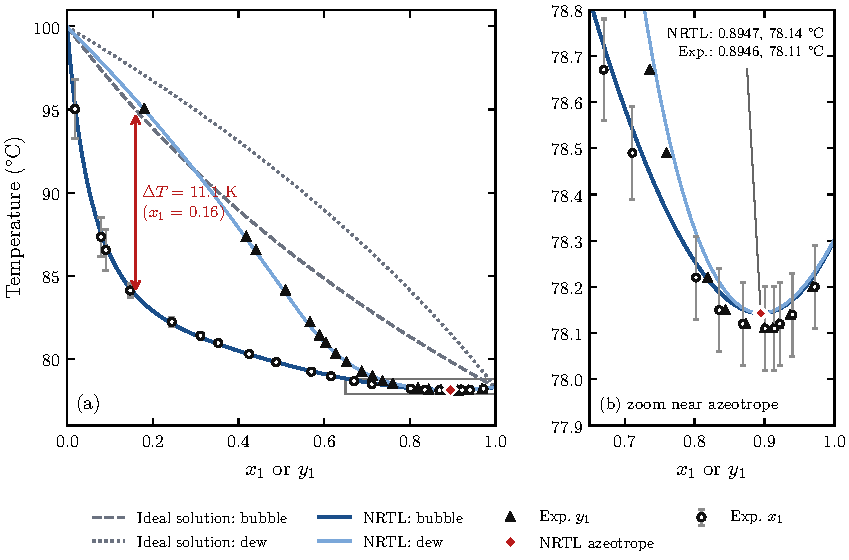
\includegraphics[width=0.9\linewidth]{../fig/fig_txy.pdf}
\caption{乙醇--水在 101.325\,kPa 的 $T$--$x$--$y$ 相圖：理想（Raoult）vs NRTL vs 實驗。(a) 全組成範圍，紅色箭頭標示泡點溫度的最大差異；(b) 共沸點附近放大。誤差棒為實驗擴展不確定度。}\label{fig:txy}
\end{figure}

\begin{figure}[!t]
\centering
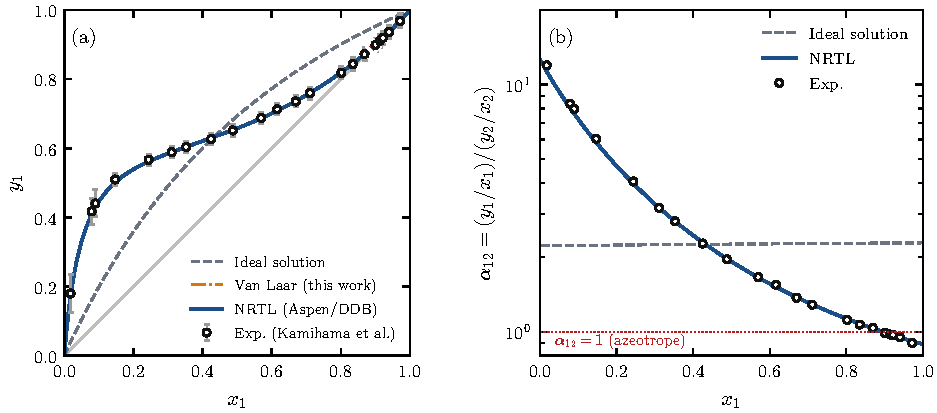
\includegraphics[width=0.84\linewidth]{../fig/fig_yx_alpha.pdf}
\caption{(a) $y$--$x$ 相圖；(b) 相對揮發度 $\alpha_{12}=(y_1/x_1)/(y_2/x_2)$（對數座標）。理想模型的 $\alpha_{12}$ 幾乎是常數（\nalphaIdLo--\nalphaIdHi），真實系統由稀端約 \nalphaMax{} 降到共沸點的 1。}\label{fig:yx}
\end{figure}

\begin{table}[H]
\centering\small
\caption{模型對 21 點實驗數據的偏差（101.3\,kPa；完整統計與殘差圖見附錄 B）。}\label{tab:stats}
\begin{tabular}{@{}lccccc@{}}
\toprule
模型 & AAD($T$)/K & max$|\Delta T|$/K & AAD($y_1$) & max$|\Delta y_1|$ & 共沸點 \\
\midrule
理想溶液（Raoult） & \naadTAAD & \nmaxTAAD & \naadyAAD & \nmaxyAAD & 無 \\
Van Laar（本研究迴歸） & \naadTVL & \nmaxTVL & \naadyVL & \nmaxyVL & $x_1=\nxAzVL$ \\
NRTL（Aspen/DDB） & \naadTNL & \nmaxTNL & \naadyNL & \nmaxyNL & $x_1=\nxAz$，\nTAz\,°C \\
實驗（內插） & — & — & — & — & $x_1=\nxAzExp$，\nTAzExp\,°C \\
\bottomrule
\end{tabular}
\end{table}

\paragraph{偏差最明顯的組成範圍。}NRTL 的 21 點全部落在實驗不確定度內；理想模型則\textbf{在稀乙醇端偏差最大}：泡點在 $x_1\approx\ndTmaxX$ 高估 \ndTmax\,K，$x_1=0.5$ 時仍有 \ndTmid\,K。原因是 $\gamma_1$ 在無限稀釋時最大（\ngOneInf），少量乙醇就使混合物蒸氣壓遠高於 Raoult 的預測。第二個偏差區在 $x_1>0.7$：真實 $\alpha_{12}$ 迅速降到 1，理想模型卻仍給 2.3。

\paragraph{若用理想模型，工程上會產生的誤判。}
\begin{enumerate}[leftmargin=1.6em]
\item \textbf{誤以為可直接蒸出高純度乙醇}：理想模型沒有共沸點，宣稱 99.5\,mol\% 只需 $R_{\min}=\nRminIdNinetyNine$；實際上常壓精餾的上限是 $x_1=\nxAz$——這就是「預期的相分離沒有發生」。
\item \textbf{能耗被系統性高估}：稀端 $\alpha_{12}$ 被低估（2.3 vs $\sim$10），$R_{\min}$ 被高估為 \nRminId（真實 \nRminNl），再沸器負荷高估 \nQBratio{} 倍（Part IV）。
\item \textbf{板數配置錯誤}：理想模型的夾點在進料，真實夾點是塔頂附近 $x\approx\npinchNl$ 的切點；理想設計把大部分板放在提餾段，精餾段嚴重不足。
\item \textbf{溫度設定點錯誤}：同組成下泡點最多差 \ndTmax\,K；把理想設計的塔放在真實相平衡下，板溫與設計值最多相差 \nTshiftMax\,K（附錄 E），控制器會持續「追錯目標」。
\end{enumerate}

% ================================================================== Part IV
\section{Excess Properties 與能量分析}\label{sec:excess}

\subsection{NRTL 計算的 \texorpdfstring{$G^{E}$}{GE} 與 \texorpdfstring{$\Delta H_{\mathrm{mix}}$}{ΔHmix}}
將\cref{eq:tau} 代入\cref{eq:gh} 得 $\Delta H_{\mathrm{mix}}$ 的解析式（推導見附錄 D），以中央差分驗證（相對誤差 $<10^{-4}$）。過剩性質應在\textbf{固定溫度}下對組成比較；沿泡點線計算時溫度隨組成改變，會把溫度效應與組成效應混在一起，因此\cref{fig:excess} 同時列出兩種結果。

\begin{figure}[H]
\centering
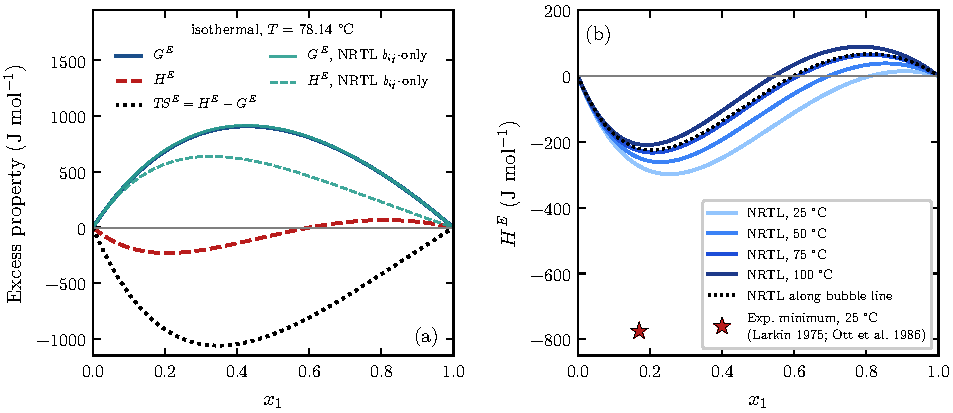
\includegraphics[width=0.9\linewidth]{../fig/fig_excess.pdf}
\caption{(a) 共沸溫度（\nTrefC\,°C）下 NRTL 的 $G^{E}$、$\Delta H_{\mathrm{mix}}=H^{E}$ 與 $TS^{E}$（淺綠為本研究另行迴歸之參數，見 4.3 節）。(b) 不同溫度下的 $\Delta H_{\mathrm{mix}}$；黑色點線為沿泡點線計算，紅星為 25\,°C 量熱實驗極小值。}\label{fig:excess}
\end{figure}

\subsection{混合為吸熱或放熱？}
\begin{answerbox}
\textbf{以放熱為主。}在 \nTrefC\,°C，$x_1<\nhEzero$ 時混合放熱（極小 \nhEmin\,J/mol，$x_1=\nhEminX$），$x_1>\nhEzero$ 時轉為輕微吸熱（極大 $+\nhEmax$\,J/mol）；$x_1=\nhEzero$ 是 $\Delta H_{\mathrm{mix}}$ 的變號點。溫度越低放熱越強：25\,°C 量熱實驗的極小值約 $-775$\,J/mol（$x_1\approx0.17$）\,\cite{larkin,ott}。
\end{answerbox}
同時 $G^{E}>0$（極大 \ngEmax\,J/mol，$x_1=\ngEmaxX$），代表混合在熱力學上「不情願」——這是正偏差與最低沸點共沸物的來源。由 $TS^{E}=H^{E}-G^{E}$，$TS^{E}$ 極小約 \nTsEmin\,J/mol：\textbf{乙醇--水的非理想性由熵主導}。乙醇加入水中形成較強的氫鍵（放熱），卻迫使水分子在乙基周圍有序排列，構型熵大幅下降（疏水水合\,\cite{frank}），淨結果仍是 $G^{E}>0$。

\subsection{模型可信度：VLE 參數不一定能預測熱效應}
25\,°C 時文獻 NRTL 預測的 $\Delta H_{\mathrm{mix}}$ 極小值為 \nhEtwoNineEightMin\,J/mol，在 $x_1=0.17$ 只有 \nhEtwoNineEightAtExp\,J/mol，\textbf{比量熱實驗低估約 2.8 倍}。我們另以同一組 VLE 數據迴歸一組 $\tau_{ij}=b_{ij}/T$ 的 NRTL 參數：它對 VLE 的擬合同樣在實驗誤差內、$G^{E}$ 幾乎重合，但預測的 $\Delta H_{\mathrm{mix}}$ 卻\emph{全組成為正}（\cref{fig:excess}a 淺綠虛線）。原因是\cref{eq:gh} 中的 $H^{E}$ 只由 $\partial(G^{E}/RT)/\partial T$ 決定，而單一等壓 VLE 只涵蓋約 17\,K 的溫度範圍，幾乎約束不了這個導數。因此混合熱的設計應以量熱數據為準。

\subsection{對混合槽／溫控設計的影響}
\begin{itemize}
\item \textbf{混合／調配槽：必須考慮。}以實驗混合熱（約 $-775$\,J/mol）與混合液熱容（約 \ncpMix\,J\,mol$^{-1}$\,K$^{-1}$）估算，25\,°C 絕熱混合可升溫約 \ndTadExp\,K（若沿用 NRTL 參數只得 \ndTadNRTL\,K）。對揮發、可燃的乙醇溶液，冷卻器應以約 10\,K 溫升設計，並在加料端設溫度聯鎖；進料溫度波動也會改變塔的 $q$ 值。
\item \textbf{蒸餾塔：混合熱可忽略。}$|\Delta H_{\mathrm{mix}}|$ 最大僅為汽化熱的 \nhEratio\%，兩成分汽化熱之比為 \ndHratio，恆莫耳溢流（CMO）成立。塔的熱負荷由汽化熱與迴流比決定，不需把混合熱納入塔換熱器 sizing。
\end{itemize}

\subsection{能量分析：再沸器負荷}
既然塔的能耗由迴流比主導，能耗誤差就來自相平衡。以 McCabe--Thiele 法（CMO，飽和液體進料，$R=\nRR\,R_{\min}$）\,\cite{seader} 比較兩種設計（\cref{fig:mccabe}、\cref{tab:design}）；NRTL 的最小迴流比由切點夾點決定：
\begin{equation}
\frac{R_{\min}}{R_{\min}+1}=\max_{x_F\le x<x_D}\frac{x_D-y^{*}(x)}{x_D-x},\qquad Q_B=\bar V\,\Delta H^{\mathrm{vap}}_{\mathrm{H_2O}}.
\end{equation}

\begin{figure}[H]
\centering
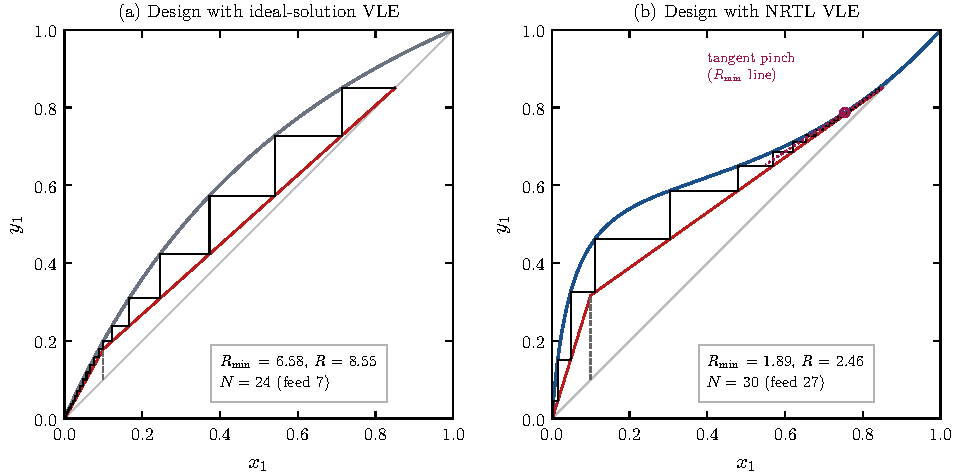
\includegraphics[width=0.78\linewidth]{../fig/fig_mccabe.pdf}
\caption{相同規格下的 McCabe--Thiele 設計：(a) 理想溶液 VLE，夾點在進料；(b) NRTL VLE，夾點為塔頂附近的切點（紫色）。}\label{fig:mccabe}
\end{figure}

\begin{table}[H]
\centering\small
\caption{設計比較（$F=\nFflow$\,kmol/h、$x_F=\nxF$、$x_D=\nxD$、$x_B=\nxB$、101.325\,kPa）。}\label{tab:design}
\begin{tabular}{@{}lcc@{}}
\toprule
項目 & 理想溶液（原設計） & NRTL（建議設計） \\
\midrule
$R_{\min}$／夾點位置 & \nRminId{}／進料（$x=\npinchId$） & \nRminNl{}／切點（$x=\npinchNl$） \\
設計 $R$；理論板數 $N$（含再沸器）；進料板 & \nRId；\nNId；第 \nNFId{} 板 & \nRNl；\nNNl；第 \nNFNl{} 板 \\
再沸器負荷 $Q_B$／冷凝器負荷 $Q_C$（kW） & \nQBId{}／\nQCId & \nQBNl{}／\nQCNl \\
比能耗（MJ／kg 乙醇） & \nEspId & \nEspNl \\
\bottomrule
\end{tabular}
\end{table}

理想模型把再沸器負荷高估 \nQBratio{} 倍——這就是「能耗預估嚴重偏差」的直接原因。諷刺的是，按理想模型建的塔即使用了更多蒸汽也達不到規格：在真實相平衡下只能做到 $x_D=\nxDach$，底部乙醇損失為設計值的 \nlossRatio{} 倍（附錄 E）。

% ================================================================== Part V
\section{顧問建議與工程判斷}\label{sec:recommend}

\subsection{此製程在目前條件下是否合理？}
\begin{answerbox}
\textbf{不合理，但可以修正。}(1) 若產品規格高於共沸組成（$x_1>\nxAz$，約 \nwAz\,wt\%），常壓蒸餾在熱力學上不可能達成；(2) 依理想模型建的塔，板數放錯位置，只能做到 $x_D=\nxDach$；(3) 溫度控制點設在對組成不敏感、對壓力很敏感的位置。只要把規格訂在共沸點以下並以 NRTL 重新設計，常壓精餾本身是成熟、合理的第一段分離。
\end{answerbox}

\subsection{哪些操作變數最敏感（\texorpdfstring{$T$、$P$、組成}{T、P、組成}）？}
\begin{table}[H]
\centering\small
\caption{操作變數敏感度（NRTL，101.325\,kPa 附近）。}\label{tab:sensop}
\begin{tabularx}{\linewidth}{@{}l>{\raggedright\arraybackslash}X>{\raggedright\arraybackslash}X@{}}
\toprule
變數 & 定量指標 & 工程意義 \\
\midrule
組成（最敏感） & 稀端 $\partial T_b/\partial x_1\approx\nsdTdxDil$\,K；精餾段僅 \nsdTdxTop\,K；$\alpha_{12}$ 由 \nalphaMax{} 降到 1 & 分離難度幾乎全集中在 $x_1>0.7$；溫度只有在稀端（提餾段）能反映組成 \\
壓力 & $\partial T_b/\partial P\approx\nsdTdP$\,K/kPa；$|\partial x^{\mathrm{az}}/\partial\ln P|\approx\nsdxazdlnP$ & 1\,kPa 的壓力波動在精餾段相當於 $\Delta x_1\approx\nsdxEquiv$ 的「假」組成變化；改變壓力幾乎移不動共沸點 \\
溫度 & 定壓下 $T$ 由組成決定，非獨立變數；$\gamma_i$ 對 $T$ 的依存弱 & 溫度是\emph{量測值}而非操控變數；混合槽的進料溫度則影響 $q$ 值 \\
\bottomrule
\end{tabularx}
\end{table}
結論：\textbf{組成是決定分離成敗的最敏感變數，壓力是干擾溫度控制的最敏感變數}。從 $x_1=0.70$ 到共沸點，板溫總共只變 \nsdTtop\,K，比 2\,kPa 壓力波動造成的變化還小；這就是現場「溫度不穩」的熱力學解釋。

\subsection{建議與熱力學理由}
\paragraph{(1) 改變操作條件——是，但不是靠改壓力。}
\begin{itemize}
\item 以 NRTL 設計：$R=\nRNl$（$1.3R_{\min}$）、\nNNl{} 塊理論板、進料移至第 \nNFNl{} 板。理由：真實夾點在塔頂切點，精餾段需要大部分板數。$R/R_{\min}=1.3$--1.5 是板數與能耗的合理折衷（$1.1R_{\min}$ 需 \nsensNa{} 板，附錄 E）。
\item 溫度控制點移到提餾段 $\partial T/\partial x$ 大的靈敏板，並採\textbf{壓力補償溫度}；塔頂組成改用線上分析或密度計。理由：精餾段溫度對組成不敏感、對壓力敏感（\cref{tab:sensop}）。
\item 產品規格訂在 $x_D\le0.85$--0.88（93.5--95\,wt\%），留距離給共沸點與切點。
\item \textbf{不建議變壓蒸餾}：10--300\,kPa 間共沸組成只從 \nxAzPTen{} 變到 \nxAzPThreeHundred；20/101.3\,kPa 組合每產出 1\,mol 乙醇至少要循環 \npsdReca\,mol（附錄 F）。理由：$x^{\mathrm{az}}$ 對 $\ln P$ 的斜率太小。
\end{itemize}

\paragraph{(2) 改用不同溶劑——乙二醇（EG）萃取蒸餾。}溶劑的作用是改變液相 $\gamma_i$ 的比值：EG 與水的親和力遠大於與乙醇，使 $\gamma_1/\gamma_2$ 上升。Kamihama 等\,\cite{kamihama} 的三元數據直接證實（\cref{fig:eg}）：近共沸區（去溶劑 $x_1'=\negXpLo$--\negXpHi、$x_{\mathrm{EG}}=\negXegLo$--\negXegHi）實驗 $\alpha_{12}=\negAlphaLo$--\negAlphaHi，無溶劑時只有 \negAlphaBinLo--\negAlphaBinHi——\textbf{共沸點被消除}。但在稀端 $\alpha_{12}$ 反而略降（\negEnhLo--\negEnhHi 倍），因此 EG 應從塔上段加入、只在高濃度區作用；EG 沸點 197\,°C，易於在回收塔分離。

\begin{figure}[!t]
\centering
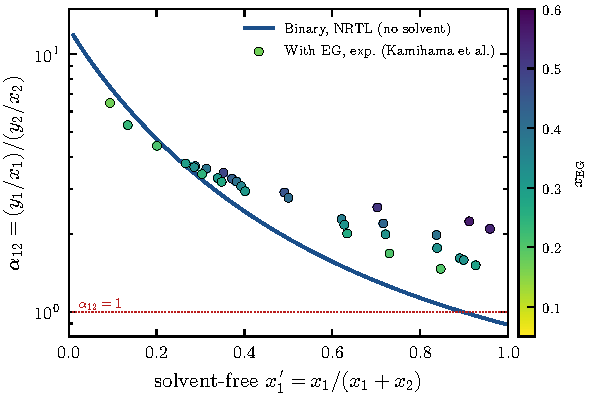
\includegraphics[width=0.44\linewidth]{../fig/fig_eg_alpha.pdf}
\caption{乙二醇對乙醇／水相對揮發度的影響（101.3\,kPa）。實線為無溶劑 NRTL；圓點為三元實驗數據\,\cite{kamihama}，顏色為液相 EG 莫耳分率。}\label{fig:eg}
\end{figure}

\paragraph{(3) 採用分段操作——建議採用。}第一段常壓精餾把乙醇濃縮到 $x_1\approx0.85$（此區 $\alpha_{12}$ 仍大、能耗低）；第二段以\textbf{分子篩變壓吸附}（3A 沸石只吸附水，不受 VLE 限制，燃料乙醇業界標準\,\cite{tereck}）或 EG 萃取蒸餾\,\cite{ignat} 跨越共沸點。理由：讓每一段只在其熱力學有利的組成區間工作，避免精餾段在 $\alpha_{12}\to1$ 的切點區耗用大量迴流。

\subsection{結論與限制}
理想溶液假設同時造成能耗高估、板數配置錯誤與溫控失效；以 NRTL 重新設計、規格訂在共沸點以下、分段完成脫水，是熱力學上最合理的路徑。限制：採 CMO 與理論板假設；$\Delta H_{\mathrm{mix}}$ 只比較 25\,°C 實驗極小值；低壓共沸點為外插。下一步應以嚴格模擬（如 Aspen Plus RadFrac）驗證\cref{tab:design}。

% ================================================================== references
\begin{multicols}{2}
\begin{thebibliography}{99}\scriptsize
\setlength{\itemsep}{0pt}\setlength{\parsep}{0pt}
\bibitem{sandler} S.\,I.\ Sandler, \textit{Chemical, Biochemical, and Engineering Thermodynamics}, 5th ed., Wiley, 2017.
\bibitem{nrtl} H.\ Renon, J.\,M.\ Prausnitz, Local compositions in thermodynamic excess functions for liquid mixtures, \textit{AIChE J.} \textbf{14} (1968) 135--144.
\bibitem{kamihama} N.\ Kamihama, H.\ Matsuda, K.\ Kurihara, K.\ Tochigi, S.\ Oba, Isobaric vapor--liquid equilibria for ethanol + water + ethylene glycol and its constituent three binary systems, \textit{J.\ Chem.\ Eng.\ Data} \textbf{57} (2012) 339--344, doi:10.1021/je2008704（數據取自 NIST TRC ThermoML）.
\bibitem{beneke} D.\ Beneke, M.\ Peters, D.\ Glasser, D.\ Hildebrandt, \textit{Understanding Distillation Using Column Profile Maps}, Wiley, 2013, Appendix B.
\bibitem{nist} P.\,J.\ Linstrom, W.\,G.\ Mallard (Eds.), \textit{NIST Chemistry WebBook}, NIST SRD 69（2026 年 10 月查閱）.
\bibitem{ambrose} D.\ Ambrose, C.\,H.\,S.\ Sprake, Thermodynamic properties of organic oxygen compounds XXV: Vapour pressures and normal boiling temperatures of aliphatic alcohols, \textit{J.\ Chem.\ Thermodyn.} \textbf{2} (1970) 631--645.
\bibitem{iapws} W.\ Wagner, A.\ Pru\ss, The IAPWS formulation 1995 for the thermodynamic properties of ordinary water substance for general and scientific use, \textit{J.\ Phys.\ Chem.\ Ref.\ Data} \textbf{31} (2002) 387--535.
\bibitem{schroeder} J.\,A.\ Schroeder, S.\,G.\ Penoncello, J.\,S.\ Schmidt, A fundamental equation of state for ethanol, \textit{J.\ Phys.\ Chem.\ Ref.\ Data} \textbf{43} (2014) 043102.
\bibitem{larkin} J.\,A.\ Larkin, Thermodynamic properties of aqueous non-electrolyte mixtures I. Excess enthalpy for water + ethanol at 298.15 to 383.15\,K, \textit{J.\ Chem.\ Thermodyn.} \textbf{7} (1975) 137--148.
\bibitem{ott} J.\,B.\ Ott, C.\,E.\ Stouffer, G.\,V.\ Cornett, B.\,F.\ Woodfield, R.\,C.\ Wirthlin, J.\,J.\ Christensen, U.\,K.\ Deiters, Excess enthalpies for (ethanol + water) at 298.15\,K and pressures of 0.4, 5, 10, and 15\,MPa, \textit{J.\ Chem.\ Thermodyn.} \textbf{18} (1986) 1--12.
\bibitem{frank} H.\,S.\ Frank, M.\,W.\ Evans, Free volume and entropy in condensed systems III, \textit{J.\ Chem.\ Phys.} \textbf{13} (1945) 507--532.
\bibitem{seader} J.\,D.\ Seader, E.\,J.\ Henley, D.\,K.\ Roper, \textit{Separation Process Principles}, 3rd ed., Wiley, 2011.
\bibitem{tereck} C.\,D.\ Tereck, Technology developments in PSA ethanol dehydration, AIChE Annual Meeting, 2006, paper 197d.
\bibitem{ignat} R.\,M.\ Ignat, A.\,A.\ Kiss, Integrated bioethanol separation and dehydration in a novel extractive DWC, \textit{Chem.\ Eng.\ Trans.} \textbf{29} (2012) 619--624, doi:10.3303/CET1229104.
\bibitem{svna} J.\,M.\ Smith, H.\,C.\ Van Ness, M.\,M.\ Abbott, M.\,T.\ Swihart, \textit{Introduction to Chemical Engineering Thermodynamics}, 8th ed., McGraw-Hill, 2018.
\bibitem{tsonopoulos} C.\ Tsonopoulos, An empirical correlation of second virial coefficients, \textit{AIChE J.} \textbf{20} (1974) 263--272.
\bibitem{herington} E.\,F.\,G.\ Herington, Tests for the consistency of experimental isobaric vapour--liquid equilibrium data, \textit{J.\ Inst.\ Petrol.} \textbf{37} (1951) 457--470.
\bibitem{coolprop} I.\,H.\ Bell, J.\ Wronski, S.\ Quoilin, V.\ Lemort, Pure and pseudo-pure fluid thermophysical property evaluation and the open-source thermophysical property library CoolProp, \textit{Ind.\ Eng.\ Chem.\ Res.} \textbf{53} (2014) 2498--2508.
\bibitem{thermo} C.\ Bell et al., \textit{thermo} and \textit{chemicals}: Chemical Engineering Design Library, \url{https://github.com/CalebBell/thermo}.
\end{thebibliography}
\end{multicols}
\label{endofmain}

% ================================================================== appendices
\clearpage
\appendix
\renewcommand{\thefigure}{\Alph{section}.\arabic{figure}}
\renewcommand{\thetable}{\Alph{section}.\arabic{table}}
\renewcommand{\theequation}{\Alph{section}.\arabic{equation}}
\renewcommand{\thesubsection}{\Alph{section}.\arabic{subsection}}

\section{計算方法與參數迴歸}\label{app:methods}
\paragraph{計算流程。}\Cref{fig:workflow} 為整體流程。正文的每一個數字都由同一套 Python 程式產生，並自動寫入 \LaTeX{} 原稿（附錄 G）。泡點以 Brent 法在 $[250,420]$\,K 求根；含汽相修正時，外層對 $\mathbf y$ 逐次代換至 $|\Delta y_1|<10^{-11}$。

\begin{figure}[H]
\centering
% Computational workflow (TikZ)
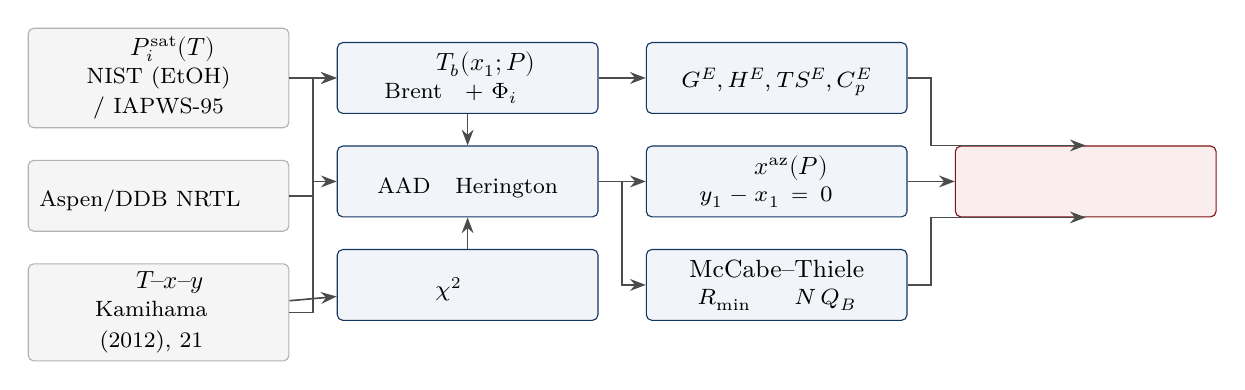
\begin{tikzpicture}[
  node distance=4mm and 6mm,
  box/.style={draw=accent!70!black, rounded corners=2pt, fill=accent!6, align=center,
              font=\small, minimum height=9mm, text width=31mm, inner sep=3pt},
  data/.style={box, fill=gray!8, draw=gray!60},
  outbox/.style={box, fill=warn!8, draw=warn!70!black},
  arr/.style={-{Stealth[length=2mm]}, semithick, draw=gray!60!black}
]
\node[data] (ant) {純物質 $P_i^{\mathrm{sat}}(T)$\\[-1pt]{\footnotesize NIST (EtOH) / IAPWS-95}};
\node[data, below=of ant] (par) {二元參數\\[-1pt]{\footnotesize Aspen/DDB NRTL；本研究迴歸}};
\node[data, below=of par] (exp) {實驗 $T$--$x$--$y$\\[-1pt]{\footnotesize Kamihama 等 (2012), 21 點}};

\node[box, right=of ant] (bub) {泡點計算 $T_b(x_1;P)$\\[-1pt]{\footnotesize Brent 法 + $\Phi_i$ 逐次代換}};
\node[box, below=of bub] (val) {模型驗證\\[-1pt]{\footnotesize AAD、殘差、Herington}};
\node[box, below=of val] (reg) {加權最小平方迴歸\\[-1pt]{\footnotesize $\chi^2$、共變異矩陣}};

\node[box, right=of bub] (exc) {過剩性質\\[-1pt]{\footnotesize $G^E,H^E,TS^E,C_p^E$}};
\node[box, below=of exc] (az) {共沸點 $x^{\mathrm{az}}(P)$\\[-1pt]{\footnotesize $y_1-x_1=0$ 求根}};
\node[box, below=of az] (mt) {McCabe--Thiele\\[-1pt]{\footnotesize $R_{\min}$（切點夾點）、$N$、$Q_B$}};

\node[outbox, right=of az] (rec) {顧問建議\\[-1pt]{\footnotesize 設計、操作、脫水方案}};

\draw[arr] (ant) -- (bub);
\draw[arr] (par.east) -- ++(3mm,0) |- (bub.west);
\draw[arr] (exp) -- (reg);
\draw[arr] (exp.east) -- ++(3mm,0) |- (val.west);
\draw[arr] (reg) -- (val);
\draw[arr] (bub) -- (val);
\draw[arr] (bub) -- (exc);
\draw[arr] (val.east) -- ++(3mm,0) |- (az.west);
\draw[arr] (val.east) -- ++(3mm,0) |- (mt.west);
\draw[arr] (exc.east) -- ++(3mm,0) |- (rec.north);
\draw[arr] (az) -- (rec);
\draw[arr] (mt.east) -- ++(3mm,0) |- (rec.south);
\end{tikzpicture}

\caption{計算流程。灰框為輸入資料，藍框為計算模組，紅框為輸出。}\label{fig:workflow}
\end{figure}

\paragraph{參數迴歸。}對 21 點數據以加權最小平方迴歸，目標函數
$\chi^2=\sum_k[(T_k^{\mathrm{calc}}-T_k^{\mathrm{exp}})/\sigma_{T,k}]^2+[(y_k^{\mathrm{calc}}-y_k^{\mathrm{exp}})/\sigma_{y,k}]^2$，$\sigma=U/2$，標準誤差由 $s^2(\mathbf J^\top\mathbf J)^{-1}$ 估計。結果：Van Laar $A_{12}=\nvlA\pm\nvlAse$、$A_{21}=\nvlB\pm\nvlBse$（相關係數 \nvlCorr，$\chi^2_\nu=\nvlChi$）；NRTL（$a_{ij}=0$、$\alpha=0.3$）$b_{12}=\nnrA\pm\nnrAse$\,K、$b_{21}=\nnrB\pm\nnrBse$\,K（相關係數 \nnrCorr，$\chi^2_\nu=\nnrChi$）。僅有單一等壓數據（78--95\,°C）時 $a_{ij}$ 與 $b_{ij}$ 幾乎共線，故只迴歸 $b_{ij}$；即使如此參數相關係數仍高達 \nnrCorr——這正是 Part IV 4.3 節 $H^{E}$ 不可辨識的根源。

\paragraph{純物質蒸氣壓檢核。}乙醇 Antoine 式（NIST，擬合範圍 292.77--366.63\,K）與 Schroeder 等\,\cite{schroeder} 參考狀態方程式（經 CoolProp\,\cite{coolprop}）比較：293--373\,K 偏差 $<\npsatDevMax\%$、393\,K 約 \npsatDevHi\%，故 1\,atm 分析延伸到 373\,K 可接受。計算常壓沸點：乙醇 \nTbEtOH\,°C、水 \nTbWater\,°C。

\section{模型驗證細節}\label{app:validation}
\paragraph{熱力學一致性。}以\cref{eq:mraoult} 由數據反算 $\gamma_i^{\exp}$，進行 Herington 等壓檢定\,\cite{herington}：
\begin{equation}
D=100\,\frac{\bigl|\int_0^1\ln(\gamma_1/\gamma_2)\,\dd x_1\bigr|}{\int_0^1|\ln(\gamma_1/\gamma_2)|\,\dd x_1}=\nherD,\qquad J=150\,\frac{T_{\max}-T_{\min}}{T_{\min}}=\nherJ,
\end{equation}
$D-J<10$，數據通過一致性檢定。

\begin{table}[H]
\centering\small
\caption{完整偏差統計（101.3\,kPa，21 點）。}\label{tab:statsfull}
\begin{tabular}{@{}lcccccc@{}}
\toprule
模型 & 汽相 & AAD($T$)/K & max$|\Delta T|$/K & 偏差($T$)/K & AAD($y_1$) & max$|\Delta y_1|$ \\
\midrule
理想溶液 & 理想氣體 & \naadTAAD & \nmaxTAAD & $+\nbiasTAAD$ & \naadyAAD & \nmaxyAAD \\
Van Laar（本研究） & 理想氣體 & \naadTVL & \nmaxTVL & $+\nbiasTVL$ & \naadyVL & \nmaxyVL \\
NRTL（本研究，$b_{ij}$） & 理想氣體 & \naadTNF & \nmaxTNF & $+\nbiasTNF$ & \naadyNF & \nmaxyNF \\
NRTL（Aspen/DDB） & 理想氣體 & \naadTNL & \nmaxTNL & $+\nbiasTNL$ & \naadyNL & \nmaxyNL \\
NRTL（Aspen/DDB） & 維里修正 & \naadTNV & \nmaxTNV & $+\nbiasTNV$ & \naadyNV & \nmaxyNV \\
\bottomrule
\end{tabular}
\end{table}

\begin{figure}[H]
\centering
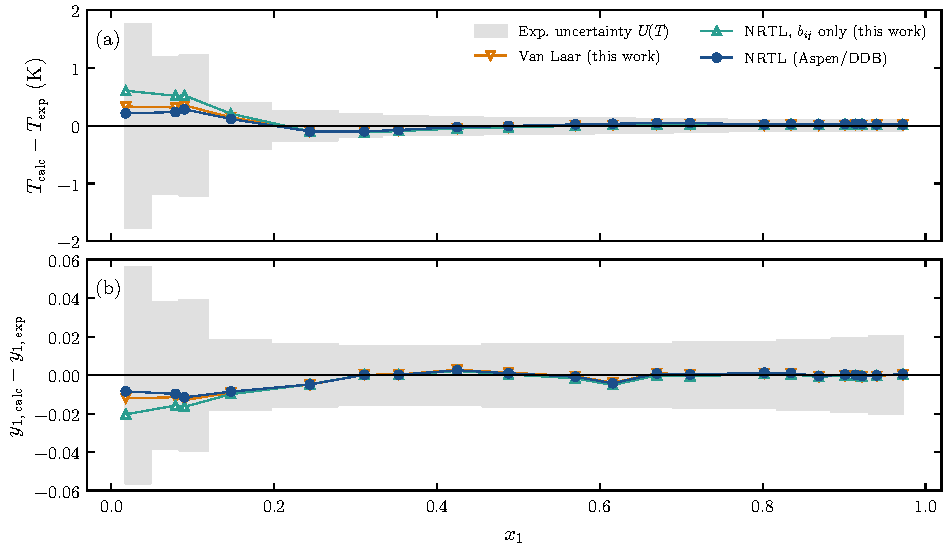
\includegraphics[width=0.9\linewidth]{../fig/fig_residuals.pdf}
\caption{泡點溫度 (a) 與汽相組成 (b) 的殘差；灰色帶為實驗擴展不確定度。理想溶液殘差（最大 \nmaxTAAD\,K）超出尺度未繪。}\label{fig:resid}
\end{figure}

\begin{figure}[H]
\centering
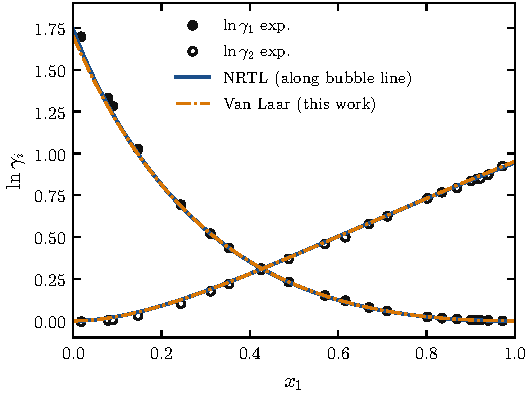
\includegraphics[width=0.55\linewidth]{../fig/fig_gamma.pdf}
\caption{由實驗反算的 $\ln\gamma_i$（點）與模型（線）。兩曲線交於 $x_1\approx0.43$，即 $G^{E}$ 極大值位置（等溫下 $\partial(G^E/RT)/\partial x_1=\ln(\gamma_1/\gamma_2)$）。}\label{fig:gamma}
\end{figure}

\begin{table}[H]
\centering\footnotesize
\caption{Kamihama 等（2012）乙醇 (1)--水 (2) 等壓 VLE，101.3\,kPa。$U$ 為擴展不確定度；$\gamma_i$ 由數據反算（含維里修正）；$\Delta$ 為 NRTL 計算值減實驗值。}\label{tab:data}
\begin{tabular}{@{}ccccccccc@{}}
\toprule
$x_1$ & $y_1$ & $T$/°C & $U(T)$/K & $U(y_1)$ & $\gamma_1$ & $\gamma_2$ & $\Delta T$/K & $\Delta y_1$ \\
\midrule
\inputtab{tab_data.tex}
\bottomrule
\end{tabular}
\end{table}

\section{汽相非理想性}\label{app:vapour}
以 $\gamma$--$\phi$ 形式 $y_i\Phi_iP=x_i\gamma_iP_i^{\sat}$，$\Phi_i=(\hat\phi_i/\phi_i^{\sat})\exp[-V_i^L(P-P_i^{\sat})/RT]$，汽相以截斷維里方程 $\ln\hat\phi_1=P(B_{11}+y_2^2\delta_{12})/RT$、$\delta_{12}=2B_{12}-B_{11}-B_{22}$ 描述\,\cite{svna}。Tsonopoulos 關聯式\,\cite{tsonopoulos} 在 351\,K 給出 $B_{11}=\nBee$、$B_{22}=\nBww$、$B_{12}=\nBew$\,cm$^3$/mol。

\begin{table}[H]
\centering\small
\caption{汽相維里修正對泡點的影響（NRTL Aspen/DDB，101.325\,kPa）。}\label{tab:virial}
\begin{tabular}{@{}ccccccc@{}}
\toprule
$x_1$ & $T_b$（理想氣體）/°C & $\Delta T$/K & $y_1$（理想氣體） & $\Delta y_1$ & $\Phi_1$ & $\Phi_2$ \\
\midrule
\inputtab{tab_virial.tex}
\bottomrule
\end{tabular}
\end{table}
修正量均小於實驗不確定度。但 Aspen/DDB 參數是在理想氣體下迴歸的，若直接加上維里修正而不重新迴歸，共沸組成會從 \nxAz{} 移到 \nxAzVir——反而偏離實驗。\textbf{活性係數參數必須與迴歸時的汽相模型搭配使用。}

\section{NRTL 混合熱的推導}\label{app:derivation}
令 $g\equiv G^E/RT=x_1x_2(f_{21}+f_{12})$，$f_{21}=\tau_{21}G_{21}/(x_1+x_2G_{21})$、$f_{12}=\tau_{12}G_{12}/(x_2+x_1G_{12})$。固定組成對 $T$ 微分：
\begin{equation}
\frac{\partial f_{21}}{\partial T}=\frac{\tau_{21}'G_{21}+\tau_{21}G_{21}'}{x_1+x_2G_{21}}-\frac{x_2\,\tau_{21}G_{21}G_{21}'}{(x_1+x_2G_{21})^{2}},\qquad
\tau_{21}'=-\frac{b_{21}}{T^{2}},\quad G_{21}'=-\alpha\,\tau_{21}'\,G_{21},
\end{equation}
$f_{12}$ 同理。代入\cref{eq:gh}：
\begin{equation}
\Delta H_{\mathrm{mix}}=H^E=-RT^{2}x_1x_2\left(\frac{\partial f_{21}}{\partial T}+\frac{\partial f_{12}}{\partial T}\right).
\end{equation}
若 $b_{ij}=0$（$\tau_{ij}$ 為常數，如課程範例程式的參數）則 $H^E\equiv0$，混合熱完全無法預測；若 $a_{ij}=0$，$G^E$ 與 $H^E$ 由同一組參數綁定而無法獨立調整——這正是 4.3 節 $b_{ij}$-only 參數 $H^E$ 符號錯誤的原因。

\section{蒸餾塔設計細節}\label{app:column}
\paragraph{理想設計在真實相平衡下的 rating。}將理想溶液設計的塔（$N=\nNId$、進料板 \nNFId、$R=\nRId$、$D/F$ 固定）放在 NRTL 相平衡下求解物料平衡：$x_D=\nxDach$、$x_B=\nxBach$；若要拉回 $x_D=\nxD$ 需 $R\approx\nRneed$、$Q_B\approx\nQBneed$\,kW。塔內溫度剖面與設計值最大相差 \nTshiftMax\,K（\cref{fig:tprofile}）。

\begin{figure}[H]
\centering
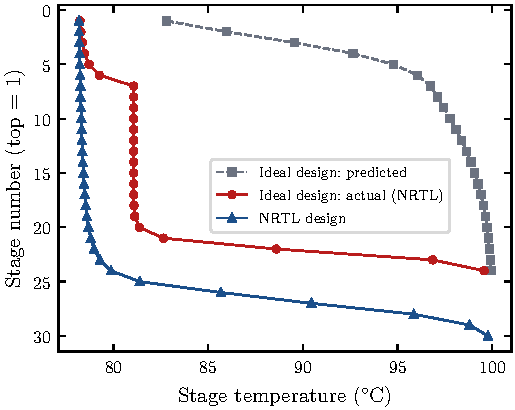
\includegraphics[width=0.55\linewidth]{../fig/fig_temperature_profile.pdf}
\caption{塔內溫度剖面。灰：理想設計的預測；紅：同一座塔在真實（NRTL）相平衡下；藍：NRTL 設計。}\label{fig:tprofile}
\end{figure}

\begin{table}[H]
\centering\small
\caption{完整設計比較與 NRTL 設計對 $R/R_{\min}$ 的敏感度。}\label{tab:designfull}
\begin{tabular}{@{}lccc@{}}
\toprule
項目 & 理想溶液 & NRTL（Aspen/DDB） & NRTL（本研究） \\
\midrule
$R_{\min}$（夾點 $x$） & \nRminId（\npinchId） & \nRminNl（\npinchNl） & \nRminNf（\npinchNf） \\
$N_{\min}$（全迴流） & \nNminId & \nNminNl & \nNminNf \\
$R$；$N$；進料板 & \nRId；\nNId；\nNFId & \nRNl；\nNNl；\nNFNl & \nRNf；\nNNf；\nNFNf \\
$\bar V$／kmol\,h$^{-1}$ & \nVId & \nVNl & \nVNf \\
$Q_B$／$Q_C$（kW） & \nQBId／\nQCId & \nQBNl／\nQCNl & \nQBNf／\nQCNf \\
塔頂／塔底溫度（°C） & \nTtopId／\nTbotId & \nTtopNl／\nTbotNl & \nTtopNf／\nTbotNf \\
\bottomrule
\end{tabular}

\vspace{6pt}
\begin{tabular}{@{}cccccc@{}}
\toprule
$R/R_{\min}$ & 1.1 & 1.2 & 1.3 & 1.5 & 2.0 \\
\midrule
$R$ & \nsensRa & \nsensRb & \nsensRc & \nsensRd & \nsensRe \\
$N$（含再沸器） & \nsensNa & \nsensNb & \nsensNc & \nsensNd & \nsensNe \\
進料板 & \nsensNFa & \nsensNFb & \nsensNFc & \nsensNFd & \nsensNFe \\
$Q_B$ / kW & \nsensQa & \nsensQb & \nsensQc & \nsensQd & \nsensQe \\
\bottomrule
\end{tabular}
\end{table}
兩組 NRTL 參數的 $R_{\min}$ 與 $Q_B$ 僅差 3--4\%：VLE 層級的參數不確定度遠小於「理想 vs 非理想」的系統性誤差。

\section{共沸點隨壓力的變化與變壓蒸餾}\label{app:psd}
\begin{figure}[H]
\centering
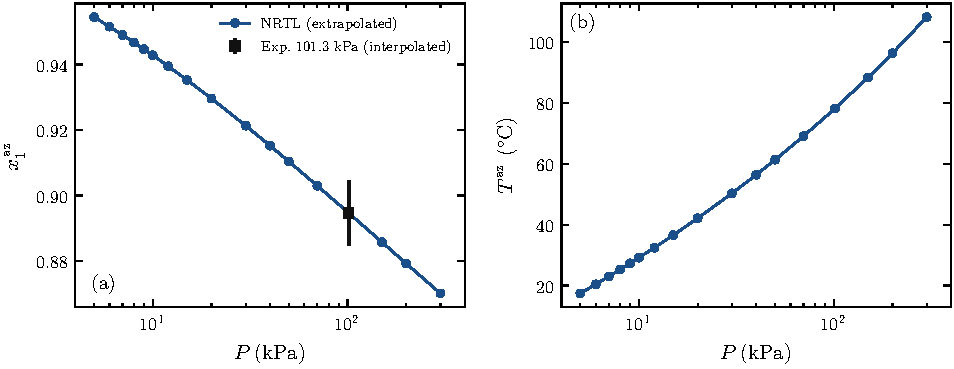
\includegraphics[width=0.9\linewidth]{../fig/fig_azeotrope_P.pdf}
\caption{NRTL 預測的共沸組成 (a) 與溫度 (b) 隨壓力的變化；參數僅由 1\,atm 附近數據決定，其他壓力屬外插；黑色方塊為 101.3\,kPa 實驗內插值。}\label{fig:azP}
\end{figure}

\begin{table}[H]
\centering\small
\caption{共沸點隨壓力變化（左）與變壓蒸餾的熱力學下限（右）。}\label{tab:azP}
\begin{tabular}[t]{@{}cccc@{}}
\toprule
$P$/kPa & $T^{\mathrm{az}}$/°C & $x_1^{\mathrm{az}}$ & wt\% \\
\midrule
\inputtab{tab_azP.tex}
\bottomrule
\end{tabular}\hspace{1.2em}
\begin{tabular}[t]{@{}lcc@{}}
\toprule
$P_L$/$P_H$ (kPa) & $\Delta x^{\mathrm{az}}$ & 最低循環比 \\
\midrule
20 / 101.3 & \npsdDxa & \npsdReca \\
10 / 101.3 & \npsdDxb & \npsdRecb \\
101.3 / 300 & \npsdDxc & \npsdRecc \\
20 / 300 & \npsdDxd & \npsdRecd \\
\bottomrule
\end{tabular}
\end{table}
最低循環比由高壓塔物料平衡 $D_{HP}/B_{HP}\ge[1-x^{\mathrm{az}}(P_L)]/[x^{\mathrm{az}}(P_L)-x^{\mathrm{az}}(P_H)]$ 求得；實際操作無法到達共沸點，循環量會更大。共沸點隨壓力的移動同樣受 $G^E$ 溫度導數控制，低壓端數值只能視為趨勢。

\section{程式與重現方式}\label{app:code}
所有計算以 Python 3（NumPy、SciPy、pandas、Matplotlib；IAPWS-95 與 Tsonopoulos 取自 \textit{chemicals}\,\cite{thermo}，蒸氣壓檢核用 CoolProp\,\cite{coolprop}）完成，置於專案儲存庫 \path{vle_consulting/report2026/}：
\begin{center}\small
\begin{tabularx}{\linewidth}{@{}l>{\raggedright\arraybackslash}X@{}}
\toprule
檔案 & 內容 \\
\midrule
\texttt{calc/vle\_core.py} & 蒸氣壓、NRTL／Van Laar、維里修正、泡點／露點、共沸點、McCabe--Thiele 與 rating \\
\texttt{calc/run\_analysis.py} & 迴歸、驗證、過剩性質、敏感度、塔設計、EG 三元分析；輸出 \texttt{results.json} \\
\texttt{calc/make\_figures.py}、\texttt{make\_numbers.py}、\texttt{make\_tables.py} & 產生圖（向量 PDF）、正文數字巨集與表格 \\
\texttt{calc/test\_core.py} & Gibbs--Helmholtz 解析式、純物質極限、共沸點 vs 實驗等測試 \\
\texttt{data/kamihama2012\_*.csv} & 二元與三元實驗數據（含來源與不確定度） \\
\bottomrule
\end{tabularx}
\end{center}
\begin{verbatim}
cd calc && python run_analysis.py && python make_figures.py \
        && python make_numbers.py && python make_tables.py
cd ../tex && xelatex report.tex && xelatex report.tex
\end{verbatim}

\end{document}
